%%%%%%%%%%%%%%%%%%%%%%%%%%%%%%%%%%%%%%%%%%%%%
% tokai-rengo-sample.tex
% 電気・電子・情報関係学会東海支部連合大会原稿 サンプルファイル(2023年版)
%%%%%%%%%%%%%%%%%%%%%%%%%%%%%%%%%%%%%%%%%%%%%

%% 本文のフォントサイズ=9pt,2段組
\documentclass[a4j,9pt,twocolumn,uplatex]{jsarticle}

\usepackage{tokai-rengo}	% 東海支部連合大会用スタイル


%% 和文題目
\title{非公式\LaTeX テンプレートによる\\令和5年度電気・電子・情報関係学会東海支部連合大会原稿の書き方}
%% 和文著者
\author{名城 太郎\DAG\PRESENTER,名城 次郎\DAG,名古屋 花子\DDAG,鈴木 秀和\DAG~(\DAG 名城大学,\DDAG ○○大学)}

%% 英文題目
\etitle{How to Write a Manuscript for the 2023 Tokai-Section Joint Conference on Electrical, Electronics, Information and Related Engineering Using Unofficial \LaTeX~Template}
%% 英文著者
\eauthor{Taro Meijo\DAG, Jiro Meijo\DAG, Hanako Nagoya\DDAG, Hidekazu Suzuki\DAG~(\DAG Meijo University, \DDAG ○○ University)}


\begin{document}

\maketitle		% タイトルの出力

\setlength{\baselineskip}{14pt} % 本文の行送りを14ptに設定

%%%%%%%%%%%%%%%%%%%%%%%%%%%%%%%%%%%%%%%%%%%%%

\section{はじめに}

毎年8月下旬から9月上旬に開催される電気・電子・情報関連学会東海支部連合大会は,原稿のテンプレートがMicrosoft Wordしか公開されていない.
そこで,令和5年度大会のフォーマットをもとに,非公式\LaTeX テンプレートを作成した.
本稿では本テンプレートの使い方を解説する.


\section{ソースファイルの構成}

\subsection{プリアンブル}
\begin{itemize}
    \item \verb|\title|,\verb|\etitle|:和文表題,英文表題
    \item \verb|\author|,\verb|\eauthor|:和文著者名・所属,英文著者名・所属
    和文著者名の姓と名の間に全角スペースを入力し,講演者の名前の後ろに\verb|\PRESENTER|を記載する.
    英文著者名の姓と名の間は半角スペースを入力する.
    著者名と所属の間にはる括弧の前に記載されている``\verb|~|''の記号は,半角空白を挿入するためのものであるため,削除しないこと.
    なお,所属が複数の場合は\verb|\DAG|,\verb|\DDAG|を用いて各著者の所属を区別すること.
\end{itemize}

\subsection{タイトルの表示}
\verb|\maketitle|によりタイトル(題目,著者,所属)が出力されるため,消さないように.

\subsection{本文}
東海支部連合大会の原稿はA4で標準1ページ,かつファイルサイズは3MB以下である必要がある.
なお,2023年度からの変更点として,ファイルサイズが3MB以下であれば2ページ以上の原稿も投稿可能になった.

\subsection{箇条書き}
番号無し箇条書きは,下記のように出力される.
\begin{itemize}
    \item 項目1
    \item 項目2
    \item 項目3
\end{itemize}

番号付き箇条書きは,括弧付きで表示されるようにスタイルファイルで設定している.
\begin{enumerate}
    \item 項目1
    \item 項目2
    \item 項目3
\end{enumerate}

\subsection{図}
\figref{fig:network}や\figref{fig:tiger}のように,PDF形式やPNG形式の図形ファイルを取り込むことができる.
キャプションは英文で記載する.

\begin{figure}[tb]
    \centering
    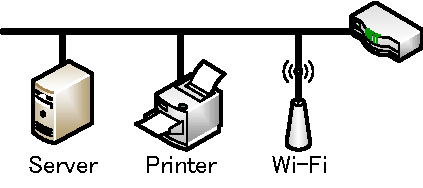
\includegraphics[width=0.5\linewidth,clip]{fig/network.pdf}
    \caption{Network configuration}
    \label{fig:network}
\end{figure}

\begin{figure}[tb]
    \centering
    
\includegraphics[scale=0.95,clip]{fig/tiger.png}
    \caption{This is a tiger}
    \label{fig:tiger}
\end{figure}

\subsection{表}
本テンプレートでは,情報処理学会論文誌の書き方に準拠して,\tabref{tab:sample}のように罫線を少なくして仕上がりをスッキリさせている.
図と同じく,キャプションは英文で記載する.
下記の点に気をつけて表を作成すること.
\begin{itemize}
    \item 表の最上部の罫線は\verb|\hline\hline|として二重線とする.
    \item 表の最下部は一重線とする.
    \item その他の罫線は見出しとデータの境界などに限定する.
\end{itemize}

\begin{table}[tb]
    \centering
    \footnotesize	% 表中のフォントサイズをfootnotesizeに設定(必ず指定すること)
    \caption{Table style based on Journal of Information Processing}
    \label{tab:sample}
    \begin{tabular}{l|lll}
        \hline\hline
         & ヘッダ1 & ヘッダ2 & ヘッダ3 \\ 
        \hline 
        項目1 & データ11 & データ12 & データ13 \\
        項目2 & データ22 & データ22 & データ22 \\  
        \hline 
    \end{tabular}
\end{table}

\subsection{図表の参照と配置}
本文から図表を参照する場合は,下記に示す独自のマクロを利用する.
これらは情報処理学会論文誌の\LaTeX テンプレートで使われるマクロと同じである.
\begin{itemize}
    \item \verb|\figref{x}|:\verb|\label{x}|を設定した図の参照
    \item \verb|\tabref{y}|:\verb|\label{y}|を設定した表の参照
\end{itemize}

図および表は段落の途中で掲載するのではなく,ページ上部か下部のどちらかに寄せて配置する.
すなわち,\verb|\begin{figure}[z]|および\verb|\begin{table}[z]|の\texttt{z}の部分には,``\texttt{t}''(上部)または``\texttt{b}''(下部)のいずれかとする.

\subsection{参考文献}
参考文献は最後の\verb|thebibliography|環境に記載する.
文献情報は\verb|\bibitem{label}|の後に,著者名,掲載誌名,巻,号,ページ,発行年などを入力する.
書き方の一例として論文誌\cite{Matsuoka2022},国際会議\cite{Suzuki2013},RFC\cite{MIPv4}を示す.


\section{まとめ}

本稿は非公式\LaTeX テンプレートに基づいて作成されている.
本稿のソースファイルをコピーして必要な箇所を修正すれば,公式テンプレートのフォーマットにほぼ準拠した原稿PDFを作成できるため,是非利用してほしい.


\subsection*{謝辞}
謝辞を記載する必要がある場合は,ここに記載する.
不要であれば\verb|\subsection*{謝辞}|ごと削除する.


%% 参考文献
\begin{thebibliography}{9}      % 文献数が1桁なら9,2桁なら99を指定
    \bibitem{Matsuoka2022} 松岡.他:情報処理学会論文誌 Vol.~63, No.~1, pp.~130--142, 2022.
    \bibitem{Suzuki2013} H. Suzuki, et al.: Proc. ACM MobiCom 2013, pp.~171--174, 2013.
    \bibitem{MIPv4} C. Perkins: RFC 5944, IETF, 2010.
\end{thebibliography}

\end{document}